\documentclass[a4paper,10pt]{article}
\usepackage{My_math_package}


\title{MATH848T - Scissors congruence, spectral sequences, Hilbert's third problem}
\author{Haoran Li}
\date{2020 Spring}

\makeindex[columns=2, title=Index, intoc] % Create the index

\begin{document}\sloppy % reduce overlong words

% Maketitle
\begin{titlepage}
\begin{center}
\vspace*{1cm}
\LARGE
\textbf{MATH848T - Scissors congruence, spectral sequences, Hilbert's third problem} \\
\vspace{2cm}
\begin{center}
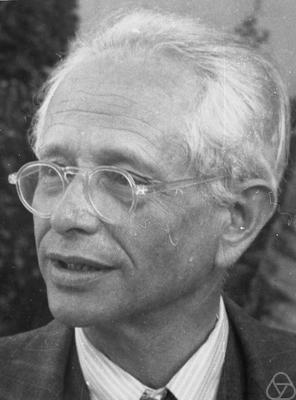
\includegraphics[width=0.5\textwidth]{Pictures/Max_Dehn.jpg}
\end{center}
\vspace{2cm}
\normalsize
Taught by \texttt{Christian Zickert} \\
Notes taken by \texttt{Haoran Li} \\
2020 Spring \\
\vspace{2cm}
Department of Mathematics\\
University of Maryland\\
\end{center}
\end{titlepage}

\tableofcontents
\newpage

\section{Hilbert's third problem - 1/28/2020}
\subfile{Hilbert's_third_problem.tex}
\newpage

\section{Scissors congruence group - 1/30/2020}
\subfile{Scissors_congruence_group.tex}
\newpage

\section{More elementary calculations on scissors congruence groups - 2/4/2020}
\subfile{More_elementary_calculations_on_scissors_congruence_groups.tex}
\newpage

\section{Spectral sequence - 2/6/2020}
\subfile{Spectral_sequence.tex}
\newpage

\section{Double chain complex - 2/11/2020}
\subfile{Double_chain_complex.tex}
\newpage

\section{Total chain complex - 2/13/2020}
\subfile{Total_chain_complex.tex}
\newpage

\section{Applications of double complex - 2/18/2020}
\subfile{Applications_of_double_complex.tex}
\newpage

\section{Cohomological spectral sequence - 2/20/2020}
\subfile{Cohomological_spectral_sequence.tex}
\newpage

\section{Exact couple - 2/25/2020}
\subfile{Exact_couple.tex}
\newpage

\section{Simplicial set - 2/27/2020}
\subfile{Simplicial_set.tex}
\newpage

\section{Group homology - 3/5/2020}
\subfile{Group_homology.tex}
\newpage

\section{Homology of abelian groups - 3/10/2020}
\subfile{Homology_of_abelian_groups.tex}
\newpage

\section{Translational scissors congruence - 3/12/2020}
\subfile{Translational_scissors_congruence.tex}
\newpage

\section{Hyperbolic scissors congruence}
\subfile{Hyperbolic_scissors_congruence.tex}
\newpage

\printindex
\newpage

\end{document}